
%% bare_jrnl_compsoc.tex
%% V1.4b
%% 2015/08/26
%% by Michael Shell
%% See:
%% http://www.michaelshell.org/
%% for current contact information.
%%
%% This is a skeleton file demonstrating the use of IEEEtran.cls
%% (requires IEEEtran.cls version 1.8b or later) with an IEEE
%% Computer Society journal paper.
%%
%% Support sites:
%% http://www.michaelshell.org/tex/ieeetran/
%% http://www.ctan.org/pkg/ieeetran
%% and
%% http://www.ieee.org/

%%*************************************************************************
%% Legal Notice:
%% This code is offered as-is without any warranty either expressed or
%% implied; without even the implied warranty of MERCHANTABILITY or
%% FITNESS FOR A PARTICULAR PURPOSE! 
%% User assumes all risk.
%% In no event shall the IEEE or any contributor to this code be liable for
%% any damages or losses, including, but not limited to, incidental,
%% consequential, or any other damages, resulting from the use or misuse
%% of any information contained here.
%%
%% All comments are the opinions of their respective authors and are not
%% necessarily endorsed by the IEEE.
%%
%% This work is distributed under the LaTeX Project Public License (LPPL)
%% ( http://www.latex-project.org/ ) version 1.3, and may be freely used,
%% distributed and modified. A copy of the LPPL, version 1.3, is included
%% in the base LaTeX documentation of all distributions of LaTeX released
%% 2003/12/01 or later.
%% Retain all contribution notices and credits.
%% ** Modified files should be clearly indicated as such, including  **
%% ** renaming them and changing author support contact information. **
%%*************************************************************************


% *** Authors should verify (and, if needed, correct) their LaTeX system  ***
% *** with the testflow diagnostic prior to trusting their LaTeX platform ***
% *** with production work. The IEEE's font choices and paper sizes can   ***
% *** trigger bugs that do not appear when using other class files.       ***                          ***
% The testflow support page is at:
% http://www.michaelshell.org/tex/testflow/


\documentclass[10pt,journal,compsoc]{IEEEtran}
%
% If IEEEtran.cls has not been installed into the LaTeX system files,
% manually specify the path to it like:
% \documentclass[10pt,journal,compsoc]{../sty/IEEEtran}





% Some very useful LaTeX packages include:
% (uncomment the ones you want to load)


% *** MISC UTILITY PACKAGES ***
%
%\usepackage{ifpdf}
% Heiko Oberdiek's ifpdf.sty is very useful if you need conditional
% compilation based on whether the output is pdf or dvi.
% usage:
% \ifpdf
%   % pdf code
% \else
%   % dvi code
% \fi
% The latest version of ifpdf.sty can be obtained from:
% http://www.ctan.org/pkg/ifpdf
% Also, note that IEEEtran.cls V1.7 and later provides a builtin
% \ifCLASSINFOpdf conditional that works the same way.
% When switching from latex to pdflatex and vice-versa, the compiler may
% have to be run twice to clear warning/error messages.






% *** CITATION PACKAGES ***
%
\ifCLASSOPTIONcompsoc
  % IEEE Computer Society needs nocompress option
  % requires cite.sty v4.0 or later (November 2003)
  \usepackage[nocompress]{cite}
\else
  % normal IEEE
  \usepackage{cite}
\fi





% *** GRAPHICS RELATED PACKAGES ***
%
\ifCLASSINFOpdf
  % \usepackage[pdftex]{graphicx}
  % declare the path(s) where your graphic files are
  % \graphicspath{{../pdf/}{../jpeg/}}
  % and their extensions so you won't have to specify these with
  % every instance of \includegraphics
  % \DeclareGraphicsExtensions{.pdf,.jpeg,.png}
\else
  % or other class option (dvipsone, dvipdf, if not using dvips). graphicx
  % will default to the driver specified in the system graphics.cfg if no
  % driver is specified.
  % \usepackage[dvips]{graphicx}
  % declare the path(s) where your graphic files are
  % \graphicspath{{../eps/}}
  % and their extensions so you won't have to specify these with
  % every instance of \includegraphics
  % \DeclareGraphicsExtensions{.eps}
\fi
% graphicx was written by David Carlisle and Sebastian Rahtz. It is
% required if you want graphics, photos, etc. graphicx.sty is already
% installed on most LaTeX systems. The latest version and documentation
% can be obtained at: 
% http://www.ctan.org/pkg/graphicx
% Another good source of documentation is "Using Imported Graphics in
% LaTeX2e" by Keith Reckdahl which can be found at:
% http://www.ctan.org/pkg/epslatex
%
% latex, and pdflatex in dvi mode, support graphics in encapsulated
% postscript (.eps) format. pdflatex in pdf mode supports graphics
% in .pdf, .jpeg, .png and .mps (metapost) formats. Users should ensure
% that all non-photo figures use a vector format (.eps, .pdf, .mps) and
% not a bitmapped formats (.jpeg, .png). The IEEE frowns on bitmapped formats
% which can result in "jaggedy"/blurry rendering of lines and letters as
% well as large increases in file sizes.
%
% You can find documentation about the pdfTeX application at:
% http://www.tug.org/applications/pdftex




\hyphenation{op-tical net-works semi-conduc-tor}

\bibliographystyle{IEEEtran}
\usepackage{amsmath}
\usepackage{amssymb}
\usepackage{amsfonts}
\usepackage{graphicx}
\usepackage{float}
\usepackage{listings}
\usepackage{xcolor}
\lstset{
  language=[pseudo]Python, % Adapté pour du pseudo-code
  basicstyle=\ttfamily, % Police de type machine à écrire
  frame=single, % Cadre autour du code
  title=\lstname, % Utilise le nom comme titre
  mathescape=true, % Permet d'utiliser des mathématiques avec $
  backgroundcolor=\color{gray!10}, % Fond légèrement coloré
  breaklines=true, % Retour à la ligne automatique
  columns=flexible, % Espacement ajusté pour les mathématiques
  keywordstyle=\color{blue}, % Couleur pour les mots-clés
  commentstyle=\color{green!50!black}, % Couleur pour les commentaires
  stringstyle=\color{red}, % Couleur pour les chaînes de caractères
}

\begin{document}
%
% paper title
% Titles are generally capitalized except for words such as a, an, and, as,
% at, but, by, for, in, nor, of, on, or, the, to and up, which are usually
% not capitalized unless they are the first or last word of the title.
% Linebreaks \\ can be used within to get better formatting as desired.
% Do not put math or special symbols in the title.

\title{Review of Reinforcement Learning and Error Models for Drone Precise Landing}

\author{Côme~PÉRIN,
        Antoine~FUSIER}% <-this % stops a space}

\IEEEtitleabstractindextext{%
% Note that keywords are not normally used for peerreview papers.
\begin{IEEEkeywords}
Neural Networks, Reinforcement Learning, Applied Computing, Engineering, Algebraic Topology
\end{IEEEkeywords}}


% make the title area
\maketitle


\IEEEdisplaynontitleabstractindextext
\IEEEpeerreviewmaketitle


%The article \emph{Reinforcement Learing and Error Models for Drone Precise Landing} \cite{studied} by %\emph{Saryazdi et al.} present a %novel framework for achieving %\textbf{Precise Drone Landing}. This %novel framework is composed of two %independent modules. The first module %operates a real-time correction of %intrinsic errors on drone position %using new error model such as %\emph{spherical error model}. The %second module consist in a %modelisation of the drone's physical %environment. This second module is %used to operate a 

\section{Introduction}\label{sec:introduction}
As the use of autonomous drones increases across sectors ranging from agriculture to package delivery, the challenges of ensuring safety for individuals and efficiency in services make autonomous landing a critical issue. This challenge has specifically been addressed in \cite{studied}, ``Using Reinforcement Learning and Error Models for Drone Precise Landing,'' published in July 2024 in the \textit{ACM Digital Library}.

The safety of autonomous landings is hindered by two types of errors: intrinsic errors arising from factors such as sensor inaccuracies \cite{jono}, control system biases, and the effects of payload \cite{Qian2020}; and extrinsic errors resulting from external forces such as wind or environmental disruptions \cite{Liu2022}.

The method proposed in \cite{studied} builds on and overcomes the specific limits of these popular limited methods (\textit{i.e.} vision-based methods \cite{Sudevan2017}) by a novel two-module framework. The first module corrects intrinsic errors with the spherical error model coupled to a real-time position correction algorithm, which can adapt to drone-specific variations without needing any extra real-time sensors like cameras \cite{studied}. The second module couples a complicated aerodynamic model with training via reinforcement learning (RL) \cite{Kober2013} to handle the problem of extrinsic errors. This way, the dynamic adjustment to external wind forces can minimize positional drift and improve precision in the landings, even in difficult conditions \cite{Liu2022}.

By enabling the coexistence of two independent modules, the framework proposed by \cite{studied} attains considerable improvements in the accuracy of landings while maintaining negligible overhead in terms of computation, hence showing the promise for real-life application both in simulated and performance environments.

\section{Context and Related Work}\label{sec:context}

Although many vision-based correction methods that use cameras and markers have been widely explored \cite{Sudevan2017}, they suffer limitations from environmental conditions such as fog, shadows, or insufficient lighting, and therefore may render them unreliable under various real-world scenarios \cite{Cocchioni2016}. Due to the mentioned limitations and drawbacks, there arises a need for stronger solutions that can work efficiently under different environmental conditions.

Machine-learning approaches have also been put forth in this direction to further improve landing accuracy, training models on large datasets to predict and correct positional errors. However, because drones are put together using different materials, it is often common even among the same models from the same manufacturer that sensors, actuators, and control systems have some intrinsic differences, thus upping the positional error. This leads to the need for a more scalable and generic method that can adapt to the variability in configurations for accurate landings \cite{Petritoli2018, 37}.

Techniques attempting to address intrinsic errors include pose estimation with markers or noise filtering by algorithms such as Kalman filters. The overall performance can be improved. However, these works often do not generalize to accommodate the broad range of biased and time-varying effects found in a real-world drone system \cite{Zhong2020}. They also do not counter disturbances or external forces that most frequently corrupt the motion of drones.

To mitigate extrinsic errors, for example due to wind, stabilization algorithms based on IMU data are widely used. While these tackle gusts, they do not directly mitigate drift due to sustained external forces \cite{41}. Using anemometers gives better wind correction, although it may be impractical because of increased cost, drag, and increased system complexity \cite{Ramanathan2022}.

Reinforcement learning (RL) approaches have shown promise in addressing internal and external challenges by training drones to adapt to their environment. Techniques such as sequential deep Q-networks and adaptive multi-level quantization models have displayed higher degrees of precision in landing within simulation scenarios. On the contrary, they usually require extensive training datasets and generalizing to diverse settings often remains a challenge \cite{Kober2013, 44}.

Due to regulatory constraints on drone testing, simulation validated these methods. Platforms like PyBullet afford realistic environments for training and evaluation, simulating aerodynamic effects, collisions, and environmental impacts. However, the absence of real-world testing puts a limit on their reliability and generalizability \cite{Panerati}.

Finally, aerodynamic modeling plays a vital role in handling external forces acting on landing. Models accounting for drag, ground effects, and wind vortex simulations have been integrated into RL frameworks allowing drones to adapt to dynamic wind conditions. Such models also enable the formulation of realistic training environments closely resembling physical environments \cite{Forster}.

The dual-module methodology proposed by Saryazdi \textit{et al.} fuses the two internal error corrections and adaptation of RL to external factors, thus providing new benchmarks for an accurate landing of drones in diverse real-world conditions.

\section{Contribution}\label{sec:contribution}
 %peut-être remplacer ci-dessous par ce qui est résumé dans l'article p3
 
 A novel framework for achieving precision landing in drones is introduced in \cite{studied}. This framework addresses the limitations of existing methods by decoupling the treatment of intrinsic and extrinsic errors into two independent modules. The key contributions of this work are outlined below.

\subsection{Intrinsic Error Correction}
A path is modeled as a function $p : [0,1] \to \mathbb{R}^3$ where $[0,1]$ stands for the flight time and $\mathbb{R}$ for the 3D-space. The internal path of the drone (its belief in its own position) is noted $p_{\text{internal}}$.

\subsubsection{Error Model Basis}
An \emph{error model} $\mathcal{P}$ is a function that takes a path and a metdata vector $m \:$ ($m : [0,1] \to \mathbb{R}^k$) then returns a modified path. The trivial error model that operates no modification over the given path is noted $\mathcal{P}_{\mathbb{I}}$.

$(\mathcal{P}_i - \mathcal{P}_{\mathbb{I}})$ is then a positional error. Thus, an approximation $\tilde{p}_{\text{true}}$ of the drone's true path can be given by \eqref{affine_comb}.

\begin{equation}\label{affine_comb}
    \tilde{p}_{\text{true}}=(\mathcal{P}_{\mathbb{I}} + \Sigma_{i=1}^{N} c_i (\mathcal{P}_i - \mathcal{P}_{\mathbb{I}}))(p_{\text{internal}}, m)
\end{equation}

Where $\forall i\in \{1, \dots, N\} \; c_i \in \mathbb{R}$

\begin{figure}[h]
    \centering
    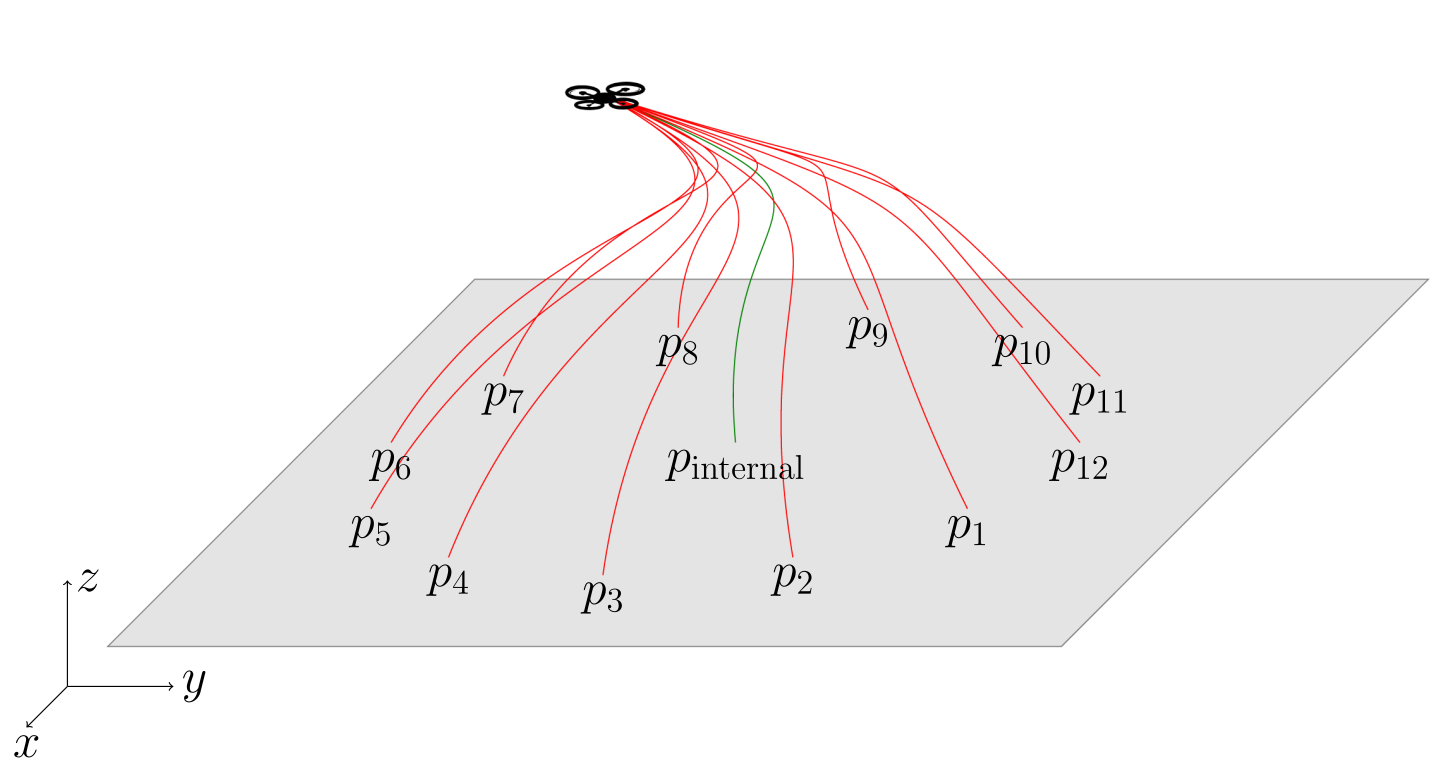
\includegraphics[width=1\linewidth]{rsc/set_error_model_paths.png}
    \caption{Example extracted from \cite{studied} of a set of error model paths $p_i~:=~\mathcal{P}(p_{\text{internal}}, m)$ for the drone’s internal position frame while landing.}
    \label{fig:enter-label}
\end{figure}

\subsubsection{Spherical Error Basis}
Observing that accumulated errors are \emph{orientation dependent}, it is possible to define a generic spherical error model basis to compute $\tilde{p}_{\text{true}}$.\cite{studied}.

Some bias ($(b_i)_i \in \mathcal{S}^2$) are chosen on the unit sphere according to \emph{Fibonacci Lattice} \cite{Hardin2016} ensuring that these points are approximately equidistant. The basis defined by \cite{studied} is presented in equation \eqref{error_basis_bias}.

\begin{equation}\label{error_basis_bias}
    (\mathcal{P}_i (p,m))(t) := p(t) + \alpha \int_{0}^{t} \left\|v_m(t') \right\| \mathrm{R}_m (t') [\mathbf{b}_i] \, dt'
\end{equation}

In Equation \eqref{error_basis_bias}, $v_m(t')$ represents the drone's velocity at time $t'$, $\alpha$ is a scaling factor empirically chosen based on the expected correction size, and $\mathrm{R}_m(t')$ is the rotation matrix transforming the bias vector $\mathbf{b}_i$ from the drone's stationary frame to its inertial position frame.

\begin{figure}
    \centering
    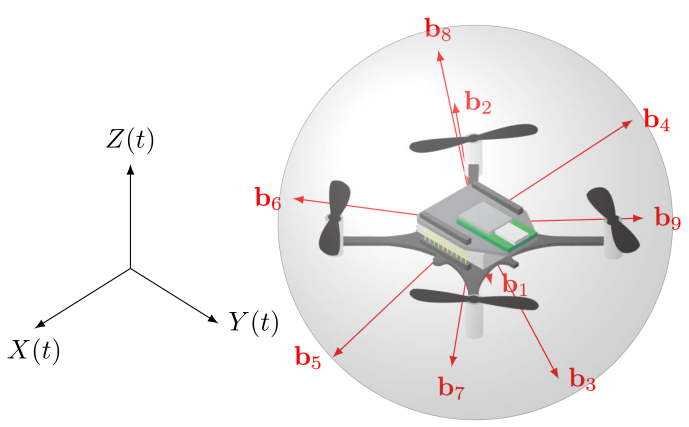
\includegraphics[width=0.7\linewidth]{rsc/bias.png}
    \caption{Example extracted from \cite{studied} of a set of bias $\mathbf{b}_i \in \mathrm{S}^2$. The stationary frame basis vectors $(X (t), Y (t), Z (t))$ are found with respect to the inertial position frame $(x, y, z)$ via a transformation by Euler angles at each time $t \in [0, 1]$}
    \label{fig:enter-label}
\end{figure}

\subsubsection{Calibration Method}
The calibration method proposed by \cite{studied} consist in sampled paths $p_k$ where $(p_k)_{\text{true}}$ and $(p_k)_\text{internal}$ are measured. Errors are then defined in \eqref{errors_def}. Note that $t=1$ is used for simplicity and no loss of generality due to $(c_i)_i$ being constant.

\begin{equation}\label{errors_def}
\begin{aligned}
    e_k &:= (p_k)_{\text{true}}(1) - (p_k)_{\text{internal}}(1), \\
    (\tilde{\mathbf{e}}_k)^i &:= ((\mathcal{P}_i - \mathcal{P}_{\mathbb{I}})((p_k)_{\text{internal}}, m))(1).
\end{aligned}
\end{equation}

Moreover, \eqref{true_equality} holds if $\tilde(p)_{\text{true}} = p_{\text{true}}$ \cite{studied}.

\begin{equation}\label{true_equality}
    \forall k \in \{1, \dots, M \} \quad \Sigma_{i=1}^{N} c_i (\tilde{\mathbf{e}}_k)^i = \mathbf{e}_k
\end{equation}

The preceding system represents a $(3M)N$ least squares linear regression problem with the unknowns $(c_i)_i$, which can be estimated in closed form using the Moore–Penrose pseudoinverse operation \cite{studied} \cite{BenGre}.

\subsubsection{Design Strategy}

This section outlines the use of the precomputed error model for live position correction.

\begin{figure}[h]
    \centering
    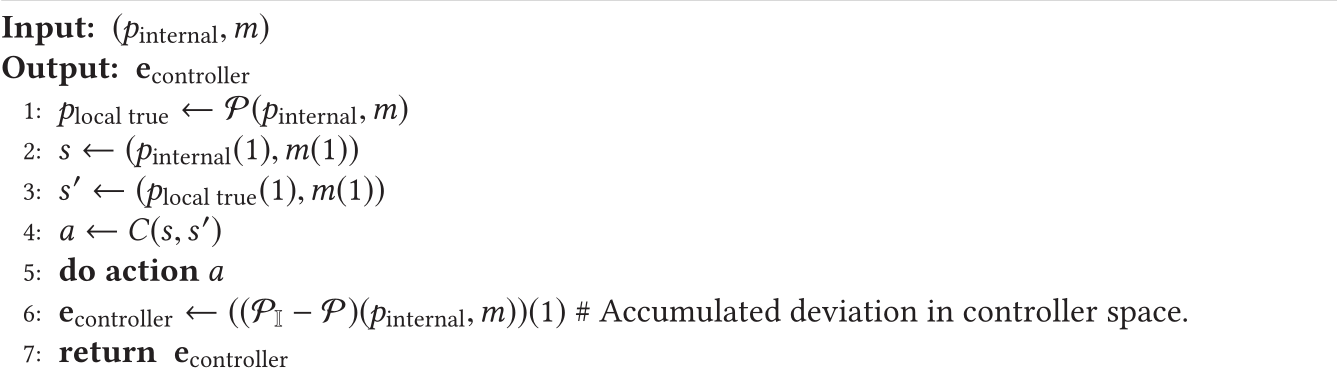
\includegraphics[width=\linewidth]{rsc/live_correction.png}
    \caption{Algorithm for Live Position Correction \cite{studied}}
    \label{fig:live_correction}
\end{figure}

Figure \ref{fig:live_correction} shows how the algorithm estimates the true path based on the internal position. Corrections are applied iteratively to align the drone's position with its true trajectory. The controller is adjusted accordingly to prevent reversion of the corrections.

\begin{figure}[H]
    \centering
    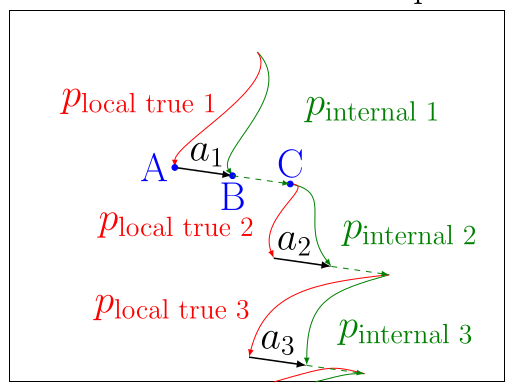
\includegraphics[width=0.4\linewidth]{rsc/trajectory_alg1.png}
    \caption{Visual representation of the internal position correction}
    \label{fig:trajectory_correction}
\end{figure}

Figure \ref{fig:trajectory_correction} illustrates the correction results. Dashed arrows indicate the predicted deviation, while solid paths represent corrected trajectories. The algorithm reduces errors over time, ensuring alignment with the true path without requiring additional sensor inputs.


\subsection{Extrinsic Error Correction}
The main purpose of this section is to train a reinforcement learning (RL) agent to face external perturbation. Strategies scalable to real cases rely on simulations that include:

\begin{itemize}
    \item \textbf{Aerodynamic modeling:} Simulations must capture forces like drag, ground effects, and wind vortices.
    \item \textbf{State space diversity:} Training must expose the agent to varied conditions and drone states.
    \item \textbf{Reward design:} The reward function should balance landing time, accuracy, and stability.
\end{itemize}

\subsubsection{Aerodynamics Model}
An aerodynamics model implementation of the Bitcraze Crazyflie
2.X drone in PyBullet Gym was used for training the RL model \cite{studied}\cite{Panerati}. However, the drag force function modelling the resistance experienced by the drone as it move through the air has been modified, partially using the work of \cite{Forster}.

\begin{equation}\label{drag_function}
    D(x,t) = -\mathbf{K_{\text{aero}}}\dot{\Theta}_{\Sigma}\mathbf{R^{-1}}(\dot{x}-W(x,t))
\end{equation}

 The drag force function from \cite{Forster} is modified by adding $\mathbf{R^{-1}}$ to account for drone orientation and $W(x,t)$ to model wind effects, enhancing aerodynamic accuracy \cite{studied}.

\subsubsection{Wind Generation Model}

A wind generation model is described in \cite{studied}, enabling the scaling of RL strategies from simulation to real-world scenarios. The wind $W(\mathbf{x},t)$ \eqref{wind} consists of several components, each is modeled using a Gaussian decaying formula $f(x,y,z,r)$ \eqref{gaussian_decay}.

\begin{equation}\label{gaussian_decay}
    f(x,y,z,r)= \exp\left(-\frac{x^2 + y^2 + z^2}{2r^2}\right) (-y, x, 0)
\end{equation}

\begin{equation}\label{wind}
\begin{aligned}
    W_i(\mathbf{x},t) &= (-1)^{o_i} \omega_{\text{max}} f(\mathbf{x}- c_i(t), r_i) \\\\
    W(\mathbf{x},t) &= \sum_{i=1}^{n} W_i(\mathbf{x},t)
\end{aligned}    
\end{equation}

In this model, $c_i(t)$ defines the center of the $i$-th wind vortex, $r_i$ its radius, and $\omega_{\text{max}}$ the maximum rotational velocity. These parameters are sampled probabilistically, with $c_i(t)$ drawn uniformly over the domain, and $r_i$ and $\omega_{\text{max}}$ sampled from predefined ranges. This ensures dynamic and varied wind conditions for better RL generalization.

\subsubsection{Reinforcement Model Methods}
To execute the RL algorithm, \cite{studied} defines the state space $\mathcal{S}$, which includes the drone's position, velocity, Euler's angles, angular velocities, and motor speeds: $s = \mathbf{(x, \dot{x}, E, \dot{E}, P)} \in \mathcal{S}$, as well as the action space $\mathcal{A}$. The actions in $\mathcal{A}$ are position difference vectors $a = (dx, dy, dz)$, which the DSLPID controller \cite{55} uses to compute the required thrust for drone orientation.

The goal of the RL algorithm is to provide a strategy that maximizes a reward function $R : \mathcal{A} \to \mathcal{S}$ \eqref{reward}:

\begin{equation}\label{reward}
\begin{aligned}
    R_1(s)&=-\frac{1}{c^2} \left\|\mathbf{x-T}\right\|^2 -1, 
    \\ 
    R_2(s)&=1-\frac{1}{2}\left(\frac{\text{max}(|\alpha|, |\beta|)}{\pi}+\frac{\text{max}(\mathbf{P})}{\mathbf{P}_\text{max}}\right)
    \\ 
    R(s) &=
\begin{cases}
    R_1(s) & \| \mathbf{x} - \mathbf{T} \| \geq c, \\
    R_1(s) + R_2(s) & \| \mathbf{x} - \mathbf{T} \| < c.
\end{cases}
\end{aligned}
\end{equation}

In the reward function \eqref{reward}, $c$ defines the threshold distance from the target $\mathbf{T}$ below which additional rewards are given. $\mathbf{P}$ represents the motor speeds, normalized by $\mathbf{P}_\text{max}$, the maximum motor speed, to penalize excessive power usage. $\alpha$ and $\beta$ denote the drone's pitch and roll angles, ensuring stability by penalizing extreme inclinations. The function encourages the drone to minimize its distance to $\mathbf{T}$ while maintaining stable angles and optimizing energy efficiency, balancing precision and control.


After initial experiments with models such as LSPI and OLSPI, the study continued with SAC (Soft Actor-Critic), which demonstrated the best results after training for 1,372 episodes. SAC effectively balances precision and robustness under varying wind intensities, ranging from $\omega_{\text{max}} = 0$ to $2$ m/s. \cite{studied}

\subsubsection{Actions}

Two approaches for drone landing actions are compared: RL-based and deterministic DSLPID. \medskip

\textbf{RL Actions} RL optimizes both accuracy and time but tends to favor speed. A rescaling trick forces precision near the target, improving accuracy in dynamic conditions like wind.

\textbf{DSLPID Actions} The DSLPID method is simple and stable, moving directly toward the target by halving the remaining distance. However, it struggles with external disturbances like wind.

\textbf{Comparison} RL adapts better to dynamic environments, offering higher precision, while DSLPID is easier to implement and performs well in controlled settings.

\subsection{Experimental Validation}
The framework’s efficacy was validated through a combination of simulation-based and real-world experiments on both modules, providing a robust demonstration of its applicability.

\subsubsection{Internal Position Correction}

Using the live correction, Figure \ref{fig:result_internal} shows that a model created with $N=500$ spherical basis model and $M=30$ data points shows in real conditions a \emph{29\% reduction in average radial differences} between the target $\mathbf{T}$ and landing point, compared to no correction \cite{studied}.

\begin{figure}[h]
    \centering
    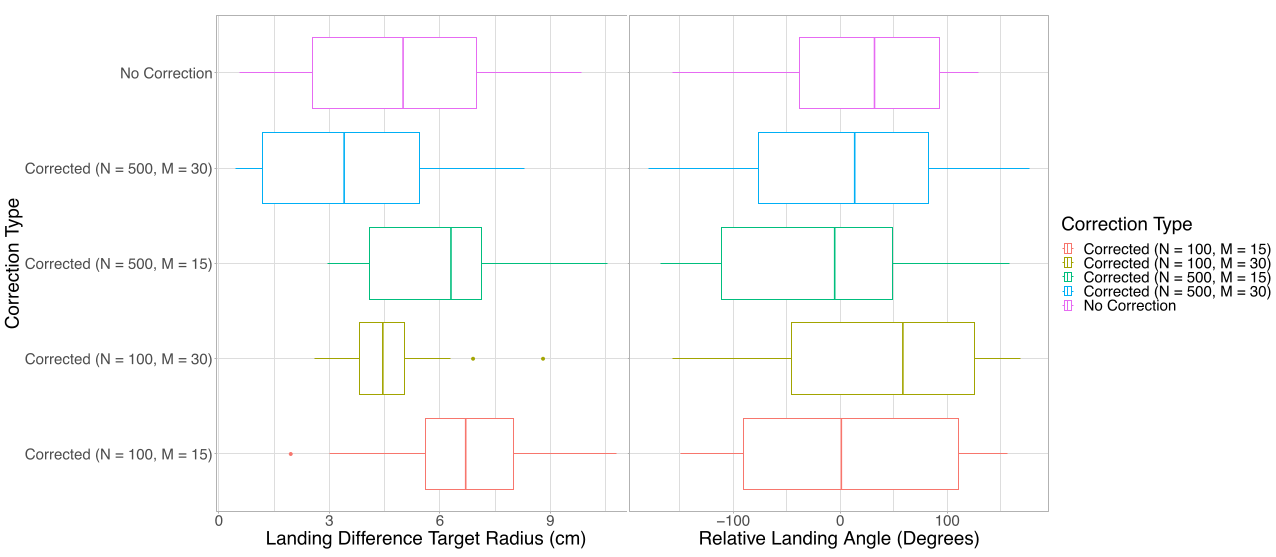
\includegraphics[width=\linewidth]{rsc/result_fig8.png}
    \caption{Result given by \cite{studied} shows distance between target \textbf{T} and the landing point for each trial by live position correction type (left) and landing angle of each trial relative to the target \textbf{T} (right).}
    \label{fig:result_internal}
\end{figure}

\subsubsection{External Position Correction}

Figure \ref{fig:external_result} shows that in real conditions, the RL strategy outperforms the straight-to-target approach only when there is wind. In calm atmosphere, the average radial distance increases by about $350\%$ in simulation, whereas in real experiments it decreases by $63\%$ under wind conditions.


\begin{figure}[h]
    \centering
    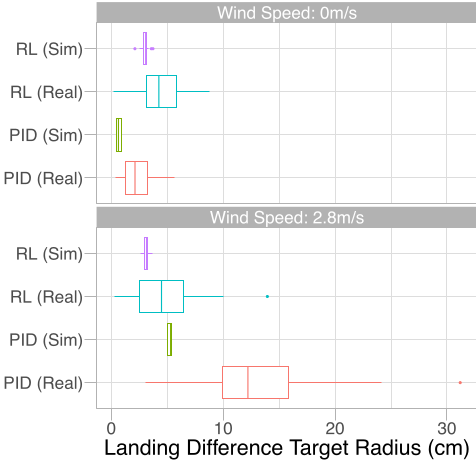
\includegraphics[width=0.6\linewidth]{rsc/external_result_fig11.png}
    \caption{Comparison of strategies by landing difference Target Radius, given by \cite{studied}}
    \label{fig:external_result}
\end{figure}

\section{Discussion}\label{sec:discussion}
Some subjects of discussion are exposed below.

\begin{itemize}
    \item \textbf{Testing modules together:} The two modules were not tested simultaneously. Would their integration introduce conflicts or affect performance in real-world scenarios?

    \item \textbf{Onboard resource requirements:} Running both modules might increase demand on the drone's CPU. Could this impact real-time responsiveness on resource-constrained hardware?
\end{itemize}



\section{Conclusion}\label{sec:conclusion}
This study presents a thorough synthesis of key findings that address one of the major challenges of landing a drone accurately and safely using a new double-module framework. This framework separates intrinsic and extrinsic error correction and embraces a spherical error model powered by reinforcement learning for significantly improved landing accuracy under a variety of conditions. Realistic modeling of aerodynamics and wind guarantees scalability to real-world application. These innovations are a big leap for autonomous drone operations, with promising applications in delivery, search and rescue, and anywhere autonomous systems need to be highly precise.
 
%\appendices


%\begin{thebibliography}{1}
\bibliography{biblio}
%\end{thebibliography}

\end{document}


